\documentclass[conference]{IEEEtran}
\IEEEoverridecommandlockouts
\usepackage{amsmath,amssymb}
\usepackage{graphicx}
\usepackage{booktabs}
\usepackage{xcolor}
\usepackage{url}
\usepackage{cite}


% Placeholder for numbers that come from ml/results/ (prints in red until filled in).
\newcommand{\res}[1]{\textcolor{red}{[TBD: #1]}}

\begin{document}

\title{RoadSense: Explainable Severity Scoring and Repair Prioritisation of Road Damage from Smartphone Images}

\author{\IEEEauthorblockN{Ninad Pandith M N}
\IEEEauthorblockA{\textit{Department of \res{department}} \\
\textit{\res{college}}\\
\res{city}, India \\
\res{email}}
\and
\IEEEauthorblockN{\res{guide name}}
\IEEEauthorblockA{\textit{Department of \res{department}} \\
\textit{\res{college}}\\
\res{city}, India \\
\res{email}}}

\maketitle

\begin{abstract}
Municipal road departments repair potholes in the order complaints arrive rather than in the order
of danger, while potholes were linked to 2,161 road deaths in India in 2023. Most research on road
damage stops at detection. We present RoadSense, a low-cost system that detects four road damage
types in smartphone photos and video with a YOLO11 detector, estimates the severity of each defect
from its size, relative monocular depth, damage type and position in the wheel path, merges
duplicate reports with a 5\,m spatial rule, and ranks repairs with an explainable priority that
adds road importance, report count, age and nearness to schools and hospitals. On the RDD2022 India
test set the detector reaches a pothole AP@0.5 of \res{E1}, and fine-tuning on \res{n} local frames
raises mAP@0.5 on a local test set by \res{E2} points. The severity score agrees with 200 hand labels
with a weighted kappa of \res{E3} on a held-out half, an ablation quantifies the contribution of
monocular depth, and merging places \res{E5} of real potholes as a single map point when a route is
surveyed twice. The system is deployed as a progressive web app with live in-browser detection and
runs on free infrastructure; code, models and a blurred local dataset are public.
\end{abstract}

\begin{IEEEkeywords}
road damage detection, pothole severity, monocular depth estimation, repair prioritisation, YOLO, edge AI
\end{IEEEkeywords}

\section{Introduction}
Potholes are the most dangerous form of road surface damage for two-wheeler riders, and in India they
were linked to 2,161 deaths in 2023 alone~\cite{morth2023}. Road departments learn about damage
through scattered complaints that are duplicated, often lack an exact location, and carry no measure
of danger; repairs therefore follow the volume of complaints rather than risk.

Smartphone images and public datasets such as RDD2022~\cite{arya2022rdd} have made automatic road
damage \emph{detection} practical~\cite{maeda2018}. Detection, however, answers only \emph{where}
damage is. A city with a limited budget needs to know \emph{how severe} each defect is and \emph{which
to repair first}, and the engineer must be able to justify that order.

This paper makes four contributions:
\begin{itemize}
\item an interpretable severity score combining size, relative monocular depth, damage type and
wheel-path position, validated against hand labels, with tuned weights and an ablation;
\item an explainable repair priority whose every term is shown to the engineer;
\item duplicate merging of citizen, rider and survey reports, evaluated by surveying a route twice;
\item a deployed, open system with in-browser detection and a published local dataset.
\end{itemize}

\section{Related Work}
Maeda et al.~\cite{maeda2018} released 9,053 smartphone images with 15,435 damage instances and
showed on-device detection; their D00/D10/D20/D40 classes became standard. RDD2022~\cite{arya2022rdd}
extends this to 47,420 images from six countries including India. Single-stage YOLO
detectors~\cite{redmon2016yolo,jocher2024yolo11} dominate because of their speed.

Beyond detection, Iqbal et al.~\cite{iqbal2022v2} convert detections into real-world measurements with
monocular depth for risk estimation, Baroudi et al.~\cite{baroudi2025} combine segmentation with depth
maps to characterise potholes, and Aburaddaha et al.~\cite{aburaddaha2026} assess detected potholes
with geometric features and a vision-language model, reporting that general monocular depth models
tend to smooth over pothole depressions. Relative depth estimators have improved
markedly~\cite{ranftl2022midas,yang2024dav2}. To our knowledge no prior system combines a validated
severity score, duplicate merging and an explainable repair ranking in a deployed application
(Table~\ref{tab:related}).

\begin{table}[t]
\caption{Comparison with related work}
\label{tab:related}
\centering
\setlength{\tabcolsep}{3pt}
\begin{tabular}{lccccc}
\toprule
Work & Detect & Severity & Merge & Rank & Deployed \\
\midrule
Maeda et al.~\cite{maeda2018} & \checkmark & -- & -- & -- & app \\
RDD2022 challenge~\cite{arya2022rdd} & \checkmark & -- & -- & -- & -- \\
Iqbal et al.~\cite{iqbal2022v2} & \checkmark & risk & -- & partly & -- \\
Baroudi et al.~\cite{baroudi2025} & \checkmark & depth & -- & -- & -- \\
Aburaddaha et al.~\cite{aburaddaha2026} & given & class & -- & -- & -- \\
\textbf{RoadSense} & \checkmark & validated & \checkmark & explained & \checkmark \\
\bottomrule
\end{tabular}
\end{table}

\section{System Overview}
\begin{figure}[t]
\centering
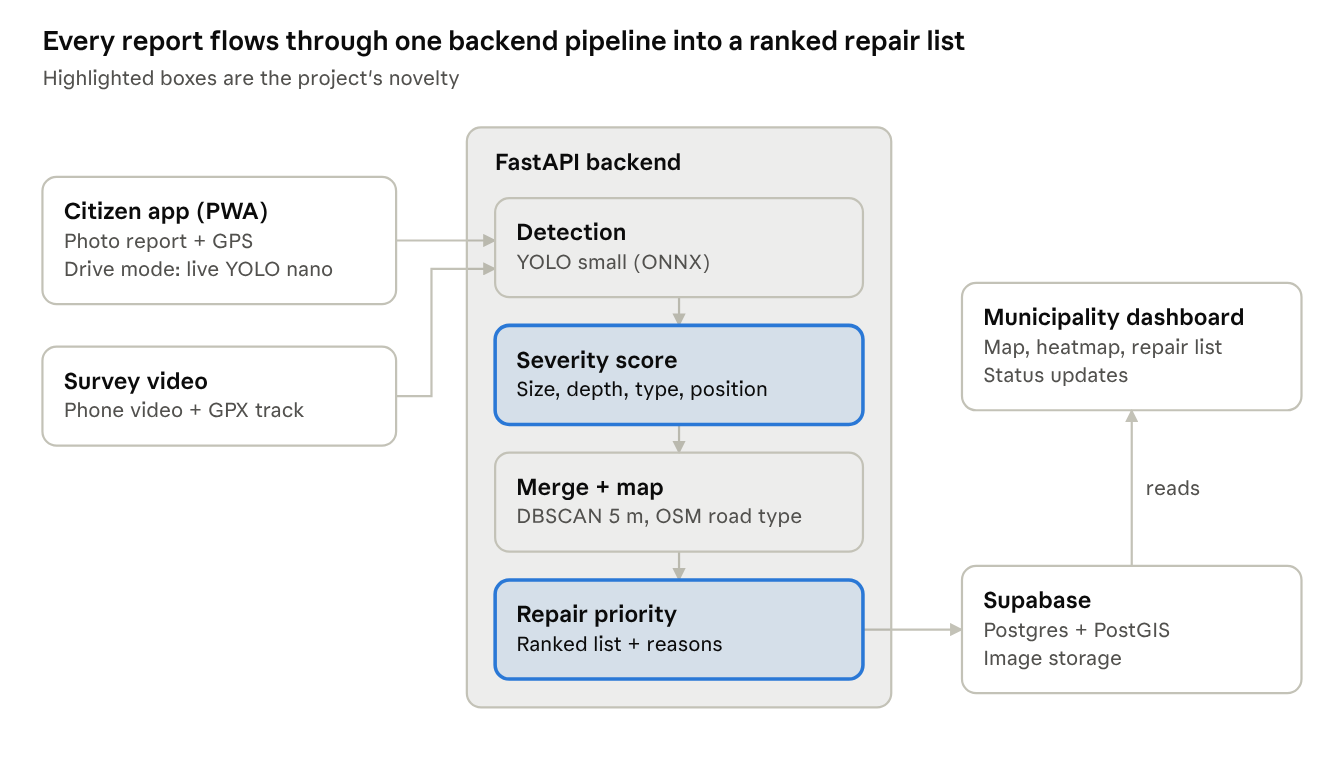
\includegraphics[width=\columnwidth]{figures/architecture.png}
\caption{RoadSense architecture. Photos, Drive-mode frames and survey videos enter one pipeline;
severity and priority turn detections into a ranked repair list.}
\label{fig:arch}
\end{figure}

Fig.~\ref{fig:arch} shows the architecture. Citizens report photos from a progressive web app;
riders use \emph{Drive mode}, in which a YOLO11n model runs in the phone browser with ONNX Runtime
Web and uploads only frames with damage; engineers upload survey videos with a GPX track, whose
frames are sampled at 4\,Hz and located by interpolating the track. Every image passes through the
same server pipeline (FastAPI, ONNX Runtime on CPU): faces and number plates are blurred in memory
before storage, YOLO11s detects damage (confidence $\geq 0.35$), each detection is scored
(Section~\ref{sec:sev}), the report is merged into a defect (Section~\ref{sec:merge}), new defects are
enriched with OpenStreetMap road class, ward and nearby schools or hospitals, and the defect's
priority is updated (Section~\ref{sec:prio}). Data lives in Postgres with PostGIS.

\section{Severity, Merging and Priority}
\subsection{Severity score}\label{sec:sev}
For a detection with normalised factors in $[0,1]$,
\begin{equation}
S = w_A A + w_D D + w_T T + w_P P,
\end{equation}
with $(w_A, w_D, w_T, w_P) = (0.35, 0.35, 0.20, 0.10)$.
\emph{Size} $A$ is the box area inside the road region (lower 55\% of the frame) relative to that
region, saturating at 20\%. \emph{Depth} $D$ uses Depth Anything V2 Small~\cite{yang2024dav2}: with
$\tilde d$ the relative inverse depth, $D = \mathrm{clip}\big((\mathrm{med}_{\text{ring}}\tilde d -
\mathrm{med}_{\text{box}}\tilde d) / (0.08\,\Delta)\big)$, where the ring surrounds the box by half
its size and $\Delta$ is the 5th--95th percentile range of $\tilde d$; a pothole floor is further away
than the surrounding road. \emph{Type} $T$ is 1.0, 0.7, 0.5, 0.4 for pothole, alligator, transverse
and longitudinal cracks. \emph{Position} $P$ is 1 within 20\% of the frame centre line and falls
linearly to 0.3 at the edge. Labels are Minor ($S<0.4$), Moderate and Dangerous ($S\geq0.7$). If
depth is unavailable, the remaining weights are renormalised.

\subsection{Duplicate merging}\label{sec:merge}
A report joins the nearest open defect within $r=5$\,m (PostGIS \texttt{ST\_DWithin} on geography),
which is the online form of DBSCAN~\cite{ester1996dbscan} with $\varepsilon=r$ and one sample per
cluster. The defect moves to the centroid of its reports and keeps the highest severity; three
reports verify it, and a report within 30 days of a repair re-opens it. Advisory locks on the grid
cells touched by the merge circle prevent concurrent reports from creating duplicates. Consecutive
detections from one ride within 2\,s are first reduced to the most confident frame.

\subsection{Repair priority}\label{sec:prio}
\begin{equation}
\Pi = S\,R\,\big(1+0.1\min(n,10)\big)\big(1+0.02\min(t,30)\big)\,B,
\end{equation}
where $R$ is road importance from the OpenStreetMap class (1.0 primary to 0.4 residential), $n$ the
number of reports, $t$ days open and $B=1.3$ within 200\,m of a school or hospital. The caps bound the
report and age boosts ($\times2$, $\times1.6$) so that neither outranks a dangerous defect on a main
road. Each term is stored and displayed with a plain-language reason, e.g.\ ``Dangerous $\cdot$ main
road $\cdot$ near school $\cdot$ 6 reports $\cdot$ 12 days open''.

\section{Implementation}
\textbf{Edge inference.} Drive mode runs YOLO11n through ONNX Runtime Web (WebGPU with a WASM
fallback) at a target of 5\,frames/s, keeps the screen awake with the Wake Lock API, and uploads
the most confident frame of each run of detections through an IndexedDB outbox that retries when
the connection returns; each report carries a client-generated identifier, so retries are
idempotent. On devices below 2\,frames/s it falls back to sending one frame every 2\,s for server
inference. The same YOLO output decoding is implemented in Python and TypeScript and tested
against identical synthetic outputs.

\textbf{Privacy.} Faces and number plates are detected and pixelated before the first write to
storage; stored images carry no EXIF, citizens need no account, and network addresses are kept only
as salted hashes for 30 days for rate limiting.

\textbf{Explainability and control.} All weights, thresholds and radii are versioned in the
database; engineers can change them, which recalculates every open priority and is logged.
Each defect page shows the photos with boxes, the four severity factors and every priority term.

\textbf{Deployment.} The web app is hosted on Vercel, the API in a scale-to-zero container on Azure
Container Apps, and data on Supabase (Postgres, PostGIS, storage, authentication, realtime), all on
free tiers. Continuous integration runs 93 backend tests against PostGIS, unit and end-to-end tests
of the web app, and automated WCAG~2 AA accessibility checks on every screen.

\section{Data and Training}
We train YOLO11 on RDD2022's labelled images (4 classes, 70/15/15 split per country, seed 42) on a
Kaggle GPU at 640\,px, then fine-tune on RDD2022 plus \res{n} frames from a \res{km}\,km pilot route
in \res{city}, recorded with a handlebar-mounted phone and a GPS logger at 1\,frame/s, de-duplicated,
pre-labelled by the base model and corrected by hand. Local frames are split by 500\,m route segment
to avoid leakage between near-identical frames. Two hundred potholes were labelled Minor, Moderate or
Dangerous before any score was viewed.

\section{Experiments}
\subsection{Detection (E1, E2)}
Table~\ref{tab:e1} compares detector sizes on the RDD2022 India test set (\res{n} images); CPU speed
is measured with ONNX Runtime at batch 1. Fine-tuning on local data changes mAP@0.5 on the local test
set (\res{n} images) from \res{before} to \res{after}.

\begin{table}[t]
\caption{Detector comparison on RDD2022 India test (E1)}
\label{tab:e1}
\centering
\begin{tabular}{lcccc}
\toprule
Model & mAP@.5 & Pothole AP@.5 & CPU FPS & MB \\
\midrule
YOLO11n & \res{} & \res{} & \res{} & \res{} \\
YOLO11s & \res{} & \res{} & \res{} & \res{} \\
YOLO11m & \res{} & \res{} & \res{} & \res{} \\
YOLOv8s & \res{} & \res{} & \res{} & \res{} \\
\bottomrule
\end{tabular}
\end{table}

\subsection{Severity agreement and ablation (E3, E4)}
Weights are tuned by grid search (step 0.05, $\sum w=1$) maximising linearly weighted
kappa~\cite{cohen1968kappa} on a stratified half of the 200 labels and evaluated on the other half
(Table~\ref{tab:e3}). The ablation removes each factor and renormalises the rest.

\begin{table}[t]
\caption{Severity versus hand labels on the held-out half (E3, E4)}
\label{tab:e3}
\centering
\begin{tabular}{lcc}
\toprule
Variant & Accuracy & Weighted $\kappa$ \\
\midrule
Original weights & \res{} & \res{} \\
Tuned weights & \res{} & \res{} \\
\midrule
without size & -- & \res{} \\
without depth & -- & \res{} \\
without type & -- & \res{} \\
without position & -- & \res{} \\
\bottomrule
\end{tabular}
\end{table}

\IfFileExists{../ml/results/e3_confusion.png}{%
\begin{figure}[t]
\centering
\includegraphics[width=0.75\columnwidth]{../ml/results/e3_confusion.png}
\caption{Severity labels from the formula versus hand labels (E3).}
\label{fig:confusion}
\end{figure}}{}

\subsection{Merging (E5) and speed (E6)}
Surveying the pilot route twice produced \res{n} reports of \res{n} real potholes. At $r=5$\,m,
\res{E5} of potholes become exactly one map point; smaller radii leave duplicates due to 5--15\,m
phone GPS error, larger radii merge neighbours (\res{sweep}). A photo report returns in \res{s}\,s
(median) on a single cloud vCPU; Drive mode runs at \res{fps}\,frames/s in a mid-range phone browser.

\IfFileExists{../ml/results/failure_grid.png}{%
\begin{figure*}[t]
\centering
\includegraphics[width=\textwidth]{../ml/results/failure_grid.png}
\caption{Failure cases: speed breakers, wet patches, shadows and water-filled potholes.}
\label{fig:failures}
\end{figure*}}{}

\section{Discussion and Limitations}
\res{Interpret E3/E4: whether depth adds agreement beyond size and type. If its contribution is small,
this is consistent with~\cite{aburaddaha2026}.} Depth is relative, so the system never reports
centimetres. The detector reflects RDD2022 and one city; speed breakers, wet patches and shadows
cause false positives. Faces and plates are blurred with classical detectors that can miss small or
angled faces. The pilot covers \res{n} defects in one area.

\section{Conclusion}
RoadSense turns smartphone images into a ranked, explained repair list by adding a validated
severity score, duplicate merging and an interpretable priority to road damage detection, and runs at
zero running cost. Future work includes vehicle-mounted city-wide surveys, predicting pothole
formation from repair history and rainfall, and integration with municipal work-order systems.
Code, models and data: \url{https://github.com/NinadPandith/Road-Sense}.

\bibliographystyle{IEEEtran}
\bibliography{refs}

\end{document}
